\chapter{Soft-Attention Visualizations}
\label{appendix:soft_attention}

Below you can find additional visualizations of the attention weights as described in Chapter~\ref{results:soft_attention}.

\begin{figure}[H]
	\centering
	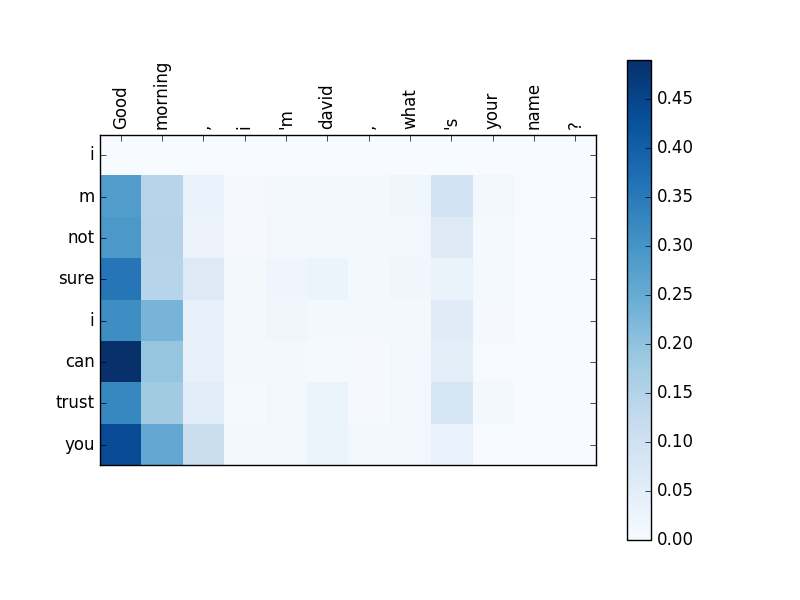
\includegraphics[width=10cm]{img/attention/attention_visualization1_OpenSubtitle-3M.png}
	\caption{Visualization of the attention weights when using the utterance ``good morning, i m david, what's your name?". On the x-axis, the input utterance is placed at the top of the chart from left to right. On the y-axis, the response from the model is placed from top to bottom. Each square in the heatmap corresponds to the attention weight the decoder computed for the thought vector of the corresponding word (x-axis) when producing the corresponding response word (y-axis). The OpenSubtitles 3.0M was used here.}
	\label{results:attention:example1:opensubtitles-3M}
\end{figure}

\begin{figure}[H]
	\centering
	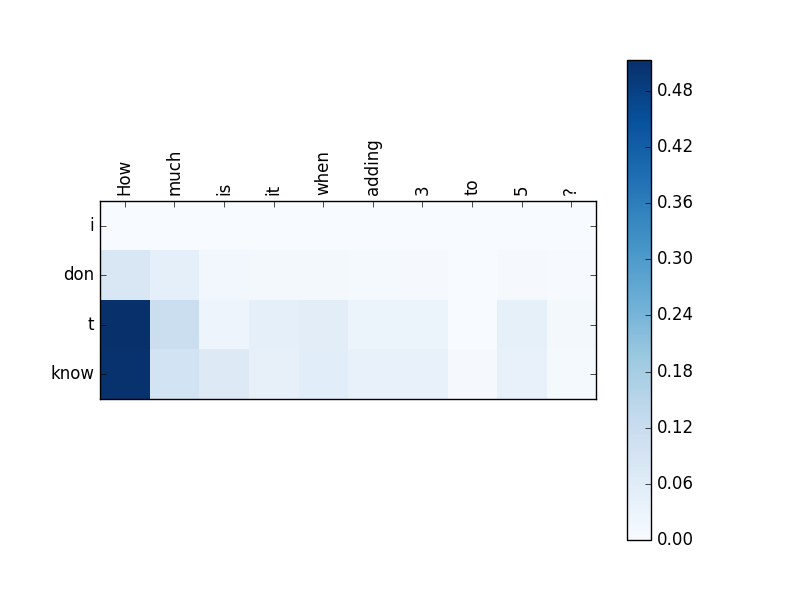
\includegraphics[width=10cm]{img/attention/attention_visualization2_OpenSubtitle-3M.png}
	\caption{Visualization of the attention weights when using the utterance ``how much is it when adding 3 to 5?". On the x-axis, the input utterance is placed at the top of the chart from left to right. On the y-axis, the response from the model is placed from top to bottom. Each square in the heatmap corresponds to the attention weight the decoder computed for the thought vector of the corresponding word (x-axis) when producing the corresponding response word (y-axis). The OpenSubtitles 3.0M was used here.}
	\label{results:attention:example2:opensubtitles-3M}
\end{figure}

\begin{figure}[H]
	\centering
	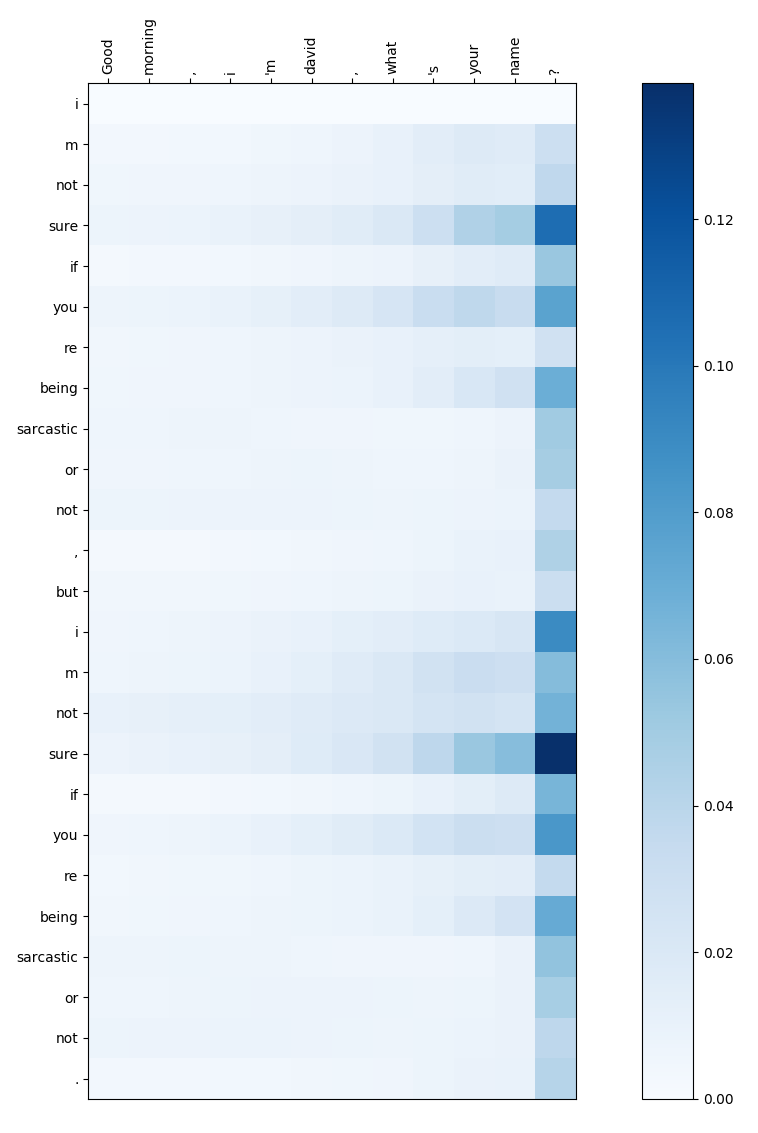
\includegraphics[width=10cm]{img/attention/attention_visualization1_reddit_2m.png}
	\caption{Visualization of the attention weights when using the utterance ``good morning, i m david, what s your name?". On the x-axis, the input utterance is placed at the top of the chart from left to right. On the y-axis, the response from the model is placed from top to bottom. Each square in the heatmap corresponds to the attention weight the decoder used on the thought vector of the corresponding word on the x-axis. The Reddit 2.0M was used here.}
	\label{results:attention:example1:reddit}
\end{figure}

\begin{figure}[H]
	\centering
	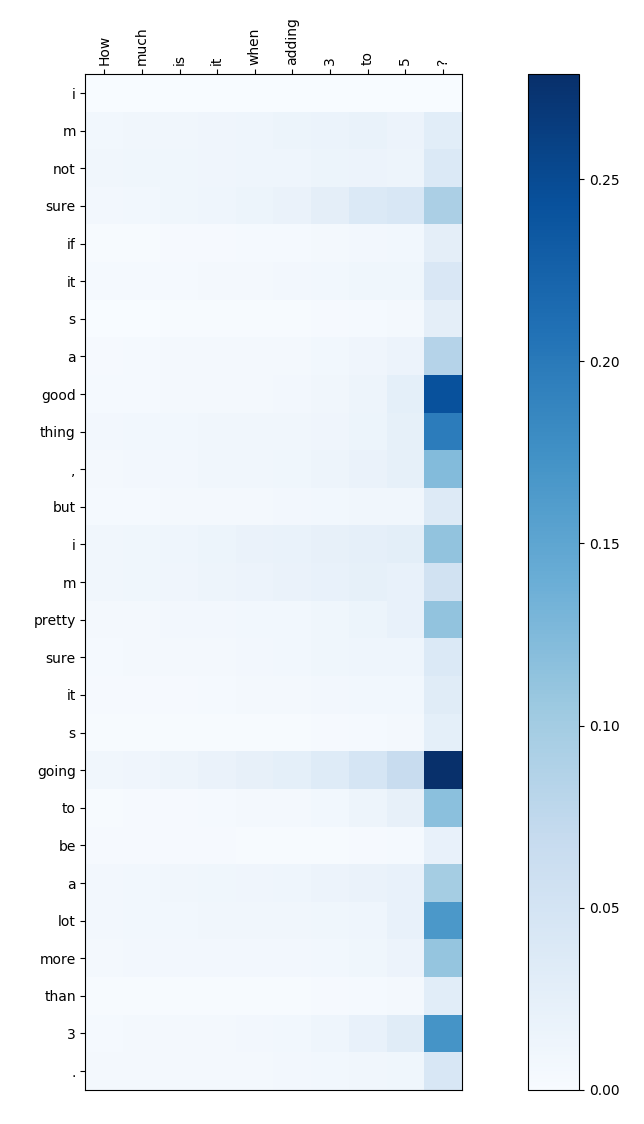
\includegraphics[width=10cm]{img/attention/attention_visualization2_reddit_2m.png}
	\caption{Visualization of the attention weights when using the utterance ``how much is it when adding 3 to 5?". On the x-axis, the input utterance is placed at the top of the chart from left to right. On the y-axis, the response from the model is placed from top to bottom. Each square in the heatmap corresponds to the attention weight the decoder computed for the thought vector of the corresponding word (x-axis) when producing the corresponding response word (y-axis). The Reddit 2.0M was used here.}
	\label{results:attention:example2:reddit}
\end{figure}

\begin{figure}[H]
	\centering
	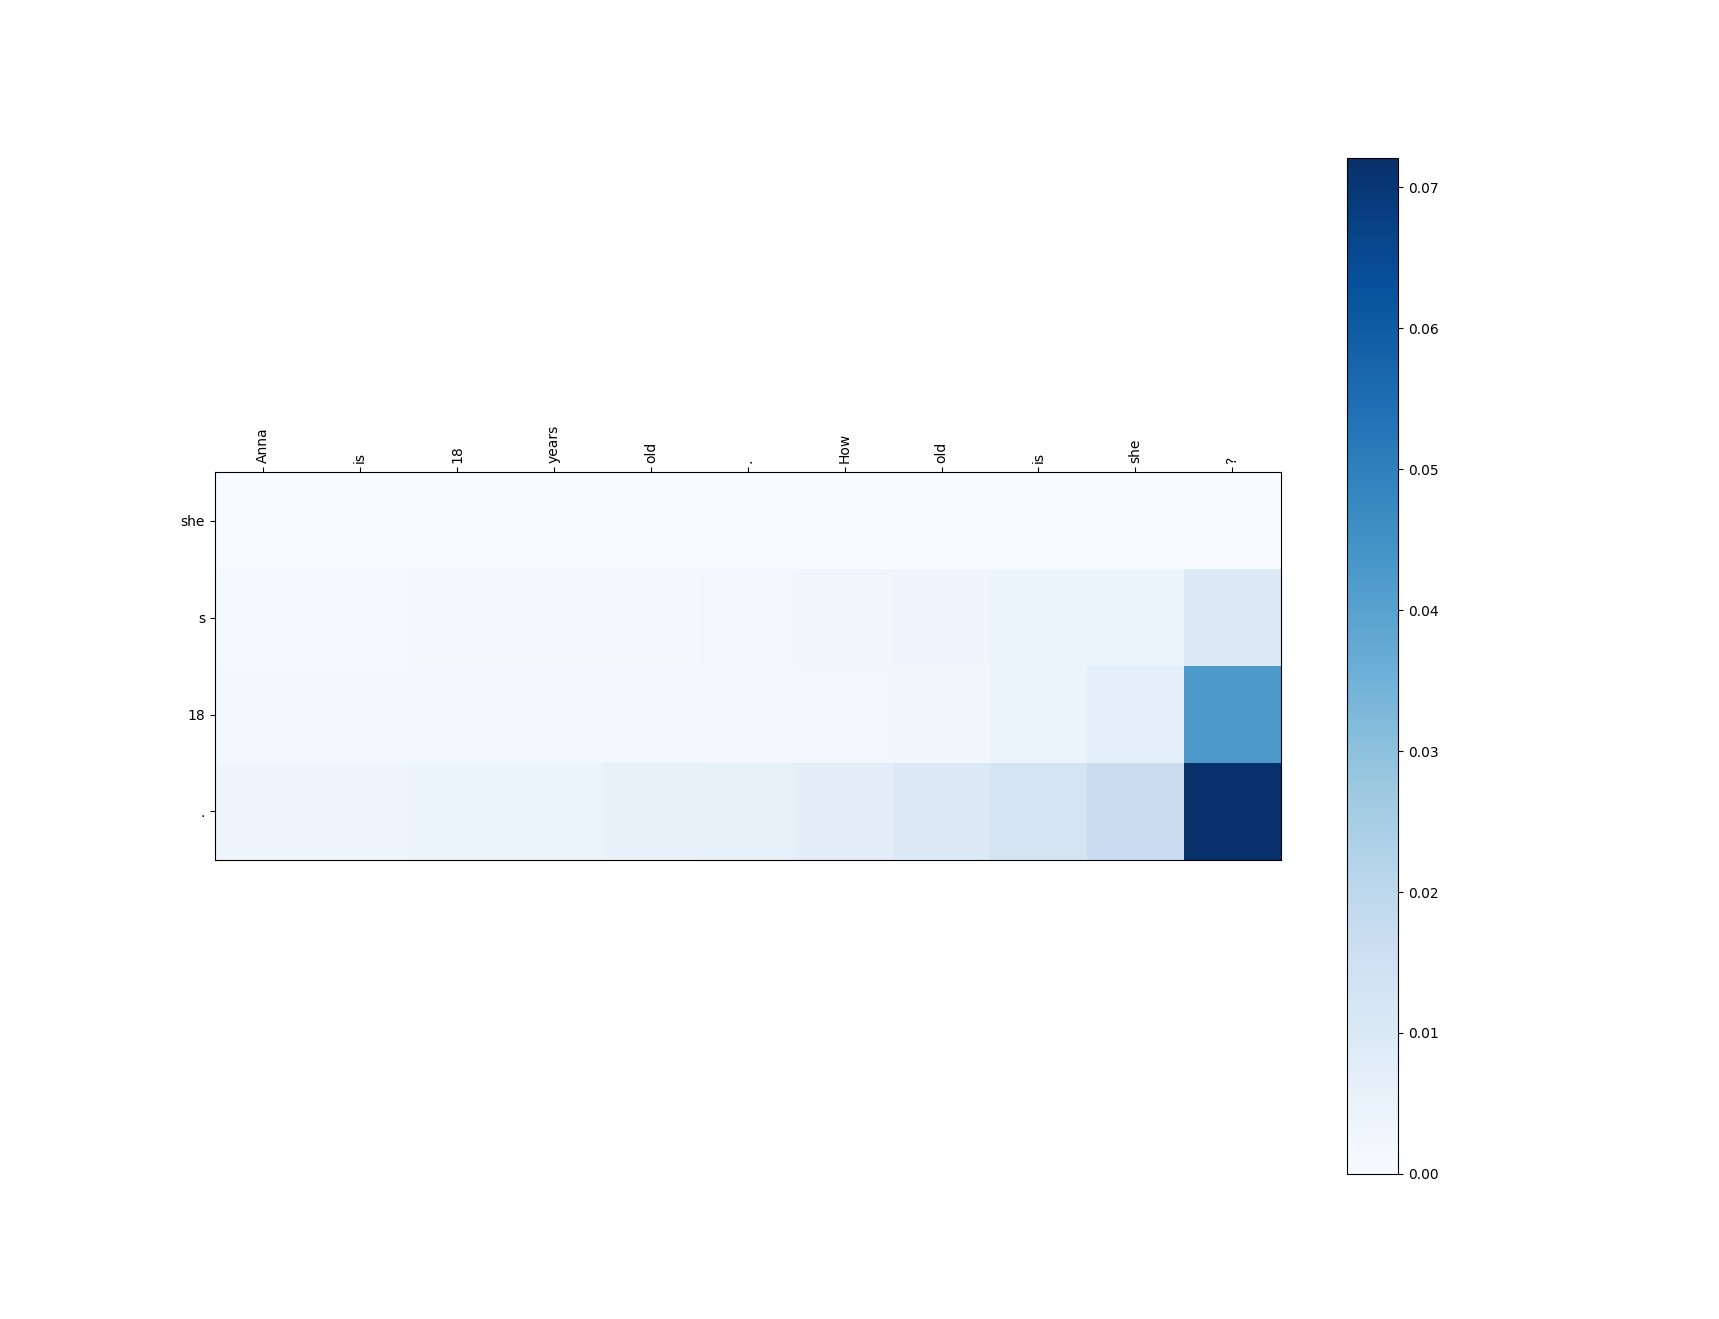
\includegraphics[width=10cm]{img/attention/attention_visualization3_reddit_2m.png}
	\caption{Visualization of the attention weights when using the utterance ``anna is 18 years old. how old is she?". On the x-axis, the input utterance is placed at the top of the chart from left to right. On the y-axis, the response from the model is placed from top to bottom. Each square in the heatmap corresponds to the attention weight the decoder computed for the thought vector of the corresponding word (x-axis) when producing the corresponding response word (y-axis). The Reddit 2.0M was used here.}
	\label{results:attention:example3:reddit}
\end{figure}